\documentclass[letterpaper,12pt]{article}
\usepackage{graphicx}
\usepackage[top=1.10in,right=1.2in,bottom=1.4in,left=1.2in]{geometry} 

\frenchspacing  % Removes extra spacing after period.

\usepackage{hyperref}

\usepackage{natbib}
%\usepackage{times}

\usepackage{amsmath}
%\usepackage{hyperref}

\usepackage{color}

\usepackage{pa}

\newcommand{\proglang}{\texttt}
\newcommand{\pkg}{\texttt}


\title{
	Evaluating Sensitivity of Parameters of Interest to Measurement Invariance in Latent Variable Models
}
\date{}

\author{\;}

\usepackage{bm}
\newcommand\vm[1]{% Vector or matrix
\bm{\mathrm{#1}}} 

\newcommand{\av}{\vm{a}}
\newcommand{\vech}{\mathrm{vech}\,}
\newcommand{\vecs}{\mathrm{vec}\,}
\newcommand{\that}{\hat{\vm{\theta}}}
\newcommand{\A}{\vm{A}}
\newcommand{\g}{\vm{g}}
\newcommand{\J}{\vm{J}}
\newcommand{\Id}{\vm{I}}
\newcommand{\Ji}{\vm{J}^{-1}}
\newcommand{\PP}{\vm{P}}
\newcommand{\da}{\textrm{{\sc {EPC}}-interest}}

\usepackage{setspace}
\doublespacing

\begin{document}
\maketitle



\begin{abstract}




\texttt{R} code and data for the examples discussed in this article are provided in the electronic appendix (\url{http://}).
\end{abstract}

\section{Introduction}



\noindent
Latent variable models are a common tool across the social sciences to model unobserved traits \citep{lord_statistical_1968,bollen_structural_1989,bartholomew2011latent}. In political science, for example, \citet{jackman2001multidimensional}  and \citet{clinton2004statistical} applied ideal point models to roll calls in the U.S. Supreme Court, Senate, and House; \citet{treier2008democracy} and \citet{armstrong2011stability} discussed measurement models for the level of democracy based on the Polity and Freedom House indicators; and \citet{davidov2009measurement} studied the measurement of national identity and constructive patriotism in the cross-national ISSP survey. The final goal of such analyses is often to compare estimated levels of the latent variable across groups; for instance, the level of democracy over time \citep{armstrong2011stability}, the risk of civil war over levels of democracy \citep{treier2008democracy}, or patriotism and nationalism over 34 countries \citep{davidov2009measurement}. Relationships between latent variables may also be compared -- for example,  the degree to which ``human value priorities'' predict attitudes against immigration across 19 European countries \citep{davidov2008values}.

Latent variables must be measured indirectly. Latent means and relationships may then only be compared across groups when group differences in these parameters of interest are unconfounded with group differences in measurement parameters \citep[e.g.][]{steenkamp_assessing_1998, oberski2012comparability}. 
One way to guarantee that differences of interest are not measurement artefacts is to establish that all (or some) measurement parameters are  equal across groups. That is, to establish (partial) ``measurement equivalence'' or ``invariance'' \citep{meredith1993measurement}, often 
using structural equation models (SEM) for continuous variables.
Chi-square difference testing \citep{steenkamp_assessing_1998,french2006confirmatory}, modification indices and expected parameter changes of the equality constraints \citep{byrne1989testing,yoon2007detecting,saris2009testing}, as well as (change in) CFI, AGFI, RMSEA, and RMR \citep{hu1998fit,cheung2002evaluating,chen2007sensitivity} are then commonly used to assess invariance model fit \citep[for reviews, see][]{millsap1993methodology,vandenberg2000review,schmitt2008measurement}.
%;closely related fields are  ``item bias'' or ``differential item functioning'' in  psychometrics \citep{mellenbergh1989item} and ``differential measurement error'' in statistics  \citep{carroll2006measurement}. 
A second way to rule out measurement artefacts as alternative explanations of substantive differences is the focus of this article: examining sensitivity,  the likely impact of measurement differences on substantive comparisons of interest.

\begin{table}[t]\centering
\begin{tabular}{lp{.2\textwidth}p{.35\textwidth}p{.35\textwidth}}
\hline
&&	\multicolumn{2}{c}{Misspecified invariance model fit}\\
	\cline{3-4}
&& ``Good'' fit & ``Bad'' fit  \\
\hline
\multicolumn{2}{l}{\emph{Conclusions}}\\
& Unaffected	 by misspecification & (1) $\surd$ & (2) Overparameterization or unnecessarily discarded item, group, or scale.\\
& Affected by misspecification & (3) Non-invariance invalidates conclusions. & (4) $\surd$\\
\hline
\end{tabular}
\caption{When the invariance model is misspecified, four situations may arise after fitting the invariance model. }\label{tab:misspecification}
\end{table}


Focusing on equality of measurement parameters and not on whether measurement equality matters for conclusions of interest  may lead to problematic situations when exact equality does not hold, as illustrated in Table \ref{tab:misspecification}. Columns in Table  \ref{tab:misspecification} represent whether invariance was rejected or not using any of the invariance evaluation procedures discussed, while rows represent the consequences for substantive comparisons of interest. 


Situations (1) and (4) in Table \ref{tab:misspecification} are unproblematic. In situation (1), the misspecifications present are inconsequential for the parameters of substantive interest, and the ``good'' model fit reflects this. Situation (1) is likely to occur when the misspecifications are small and the conclusions are not sensitive to the misspecifications in question. In situation (4), the misspecifications would have invalidated substantive comparisons if left undetected, but the model fit evaluation has correctly signaled their presence, which will tend to occur when misspecifications are large and the parameters of interest sensitive to them.

In contrast, situations (2) and (3) in Table \ref{tab:misspecification} can seriously harm inference. While misspecifications may be present and even appear substantial, the parameters of interest are not necessarily sensitive to them (situation 2).
  An -- arguably worse -- situation occurs in situation (3). Here, fit indices signal a ``close fit'', but, due to large sensitivity, even ``small'' misspecifications  substantially change parameters of interest. In this situation, even though an invariance model may appear to fit well, measurement artefacts still invalidate  comparisons of substantive interest: precisely the problem that invariance testing was intended to prevent.



To prevent unnecessary information loss or a false sense of security when comparing groups using latent variables, invariance testing (columns of Table \ref{tab:misspecification}) should thus be supplemented with sensitivity analysis (rows of Table \ref{tab:misspecification}). 
This article suggests using the ``EPC-interest'' for that purpose: a measure of the expected change in the parameter of interest
when freeing a particular equality restriction \citep{satorra1989alternative,bentler1992some}. Given parameters of interest to be compared across groups, the $\da{}$ allows the researcher
to establish more directly whether such a comparison is valid. Re-analyses of published examples show that both problematic situations (2) and (3) arise in practice, and how the $\da$ can be used to prevent needless information loss and warn of otherwise unnoticed threats to cross-group comparisons. 

The $\da{}$ is different from the well-known ``expected parameter change'' (EPC)  introduced to structural equation modeling by \citet{saris_detection_1987}. When considering what, hypothetically, can be expected to happen after freeing an equality constraint on a measurement parameter, the EPC estimates the expected change in that same measurement parameter, whereas the $\da{}$ estimates the expected change in the parameter(s) of interest.
It thus evaluates the sensitivity of the substantive model of interest to the invariance restrictions, and is similar in spirit to the approach for causal inference discussed by \citet[pp. 552-3]{imai2010causal}. The $\da$ approach also differs somewhat from the purely derivative-oriented approach to sensitivity analysis  common in econometrics \citep[p. 168]{magnus2007local} and applied to SEM by \citet{yuan2003assessing}: both direction and magnitude of the misspecification are combined into the same measure here. A contingent hypothesis test of no change in the parameters of interest is, however, equivalent to classic econometric specification tests \citep{yuan2003assessing,hausman1978specification}. Changes in parameters of interest for specific combinations of measurement and structural models were derived by  \citet{millsap1997invariance}, \citet{millsap2004evaluating}, \citet{millsap2007invariance}, and \citet{meuleman2012item}. The $\da$ can be seen as a general method of obtaining such results applicable to all structural equation models with equality-constrained measurement parameters.


\vspace{12pt}
The following section 
defines the $\da$ for structural equation models with equality
constraints. Subsequently, a simulation study evaluates the finite sample performance
of the $\da$ as an estimate of the shift in parameters of interest when freeing
misspecified equality restrictions, as well as its robustness to misspecification in the alternative model. Sections \ref{sec:app1},  \ref{sec:app2} and \ref{sec:app3} demonstrate the
use of the $\da$ on three latent variable analyses from the literature where comparisons across groups were of interest (see the digital appendix for \texttt{R} code and data\footnote{Please see the author's Dataverse study \url{http://hdl.handle.net/1902.1/21816}}). 
The final section summarizes the findings and discusses some  limitations
and  future work on the use of the $\da$ for evaluating invariance hypotheses.


\section{Assessing the effect of misspecified invariance restrictions on 
	SEM parameters of interest}

A structural equation model is any model $\boldsymbol\Sigma(\boldsymbol\theta), \boldsymbol\mu(\boldsymbol\theta)$ that imposes a structure on the population covariance matrix $\boldsymbol\Sigma$ and mean vector $\boldsymbol{\mu}$ of observed variables $\boldsymbol{y}$ as a function
of a vector $\boldsymbol\theta$ of unknown model parameters \citep{bollen_structural_1989}.
A common parameterization of SEM is the LISREL ``all-y''  model for group $g$, 
\begin{eqnarray}
	\boldsymbol{y}_g &=& \boldsymbol{\nu}_g + \boldsymbol\Lambda_g \boldsymbol\eta_g + \boldsymbol\epsilon_g,\\
	\boldsymbol{\eta}_g &=& \boldsymbol{\alpha}_g + \mathbf{B}_g \boldsymbol\eta_g + \boldsymbol\zeta_g,
\end{eqnarray}
where $\boldsymbol{\eta}_g$  is a vector of latent variables, and $\boldsymbol{\epsilon}_g$ and  $\boldsymbol{\zeta}_g$ are observed and latent variable residuals. The ``measurement model'' consists of the first equation involving as parameters the vector of intercepts $\boldsymbol{\nu}_g$, the loading matrix $\boldsymbol{\Lambda}_g$, and the residual variance matrix $\mathrm{Var}(\boldsymbol{y}_g | \boldsymbol{\eta}_g) = \mathrm{Var}(\boldsymbol{\epsilon}_g) := \boldsymbol{\Psi}_g$. The second equation is the ``structural'' part of the model with 
latent intercepts (or means) $\boldsymbol{\alpha}_g$, latent variable regression coefficients $\boldsymbol{B}_g$, and the (residual) variance matrix $\mathrm{Var}(\boldsymbol{\zeta}_g) := \boldsymbol{\Phi}_g$ as group-specific parameters. Assuming $\boldsymbol{\eta}$, $\boldsymbol{\epsilon}$, and $\boldsymbol{\zeta}$ are mutually uncorrelated, this model produces as moment structure implications
\begin{equation}
\boldsymbol\Sigma(\boldsymbol{\theta}) = \boldsymbol\Lambda (\Id - \mathbf{B})^{-1} \boldsymbol\Phi (\Id - \mathbf{B})^{-T} 
\boldsymbol\Lambda' + \boldsymbol\Psi,
\end{equation}
for the covariances and 
\begin{equation}
\boldsymbol\mu(\boldsymbol\theta) = \boldsymbol{\nu} + \boldsymbol\Lambda (\Id - \mathbf{B})^{-1} \boldsymbol{\alpha} 
\end{equation}
for the means, where for notational convenience  the group-specific parameters have been stacked to obtain the block-diagonal covariance matrix over all groups. 

Estimation of the parameters $\mathbf{a} = [\boldsymbol{\nu}',\boldsymbol{\alpha}',(\vecs \boldsymbol\Lambda)', (\vech \boldsymbol\Phi)', (\vecs \mathbf{B})', (\vech \boldsymbol\Psi)']'$ then proceeds by  minimizing a nonnegative fitting function $F(\mathbf{S}, \mathbf{m}; \boldsymbol\Sigma(\boldsymbol\theta), \boldsymbol\mu(\boldsymbol\theta))$ so that 
$\that = {\arg \min}_{\boldsymbol\theta} F(\mathbf{S}, \mathbf{m}; \boldsymbol\Sigma(\boldsymbol\theta), \boldsymbol\mu(\boldsymbol\theta))$ \citep[e.g.][]{satorra1989alternative}. A common choice of fitting function is that corresponding
to maximum likelihood estimation under the assumption that  $\mathbf{y}$ is independently and identically distributed as multivariate normal \citep{bollen_structural_1989}. Under the model, however, such distributional assumptions do not affect consistency of the parameter estimates \citep{satorra1989alternative}.

Models freely estimating all parameters in $\av$  are generally not identifiable. Therefore, restrictions $\av = \av(\boldsymbol{\theta})$ are imposed, such as setting certain loadings to zero, restricting the residual variance matrices to be diagonal, or allowing only recursive latent variable regression coefficients.  Any subset of $\av$ may play the role of the parameter interest; attention may focus on differences in the latent means $\boldsymbol{\alpha}_g$ over groups $g$, for instance, or on differences in latent variable regressions $\mathbf{B}_g$. Although there is in principle no restriction on what may defined as a parameter of interest, often the parameters of direct interest are the structural parameters \citep{fan2006impact}.

To identify differences over groups in structural parameters pertaining to latent variables, however, it is necessary to impose cross-group equality restrictions on the measurement parameters: the measurement invariance restrictions. Even when no explicit restrictions are made, but, for instance, one loading is set to unity in each group to identify regression coefficients in each group, the assumption of invariance of such reference loadings is implicit \citep{hancock2009tenuousness}. For identifiability of the comparison of interest, then, it is necessary to include in the restrictions $\av = \av_0(\boldsymbol{\theta})$ equality restrictions on the measurement model. In general, equality of loadings $\boldsymbol{\Lambda}_{g'} = \boldsymbol{\Lambda}_{g} \forall g \neq g'$ (``metric invariance'') is required for identification of parameters pertaining to the covariance matrix of the latent variables such as $\mathbf{B}_g$, while for identification of latent mean differences in $\boldsymbol{\alpha}_g$, equality of both loadings and intercepts $\boldsymbol{\Lambda}_{g'} = \boldsymbol{\Lambda}_{g};  \boldsymbol{\nu}_{g'} = \boldsymbol{\nu}_{g} \forall g \neq g'$  (``scalar invariance'') is required. Of course, such restrictions may be misspecified, and the misspecifications may cause bias in the parameters of interest \citep{yuan2003assessing,millsap2007invariance,kolenikov2009biases}. It is not necessary that the full measurement parameter vectors be equal however: partial invariance of at least two indicators per latent concept suffices for identification of the parameters of interest \citep{byrne1989testing}. This suggests that after estimation of a fully invariant model with restrictions $\av_0(\boldsymbol{\theta})$, a partially invariant alternative model $\av_a(\boldsymbol{\theta})$ can be considered which frees one equality restriction. Alternatively, $\av_0(\boldsymbol{\theta})$ may itself be a partially invariant model, assuming that it and the alternative model remain identifiable.

The $\da$ of an equality-constrained measurement parameter with respect to a 
parameter of interest in the $\av_0$ model is defined as a consistent estimate of the expected 
change in the parameter of interest if the equality constraint were freed in the $\av_a$ model.
Let the parameters of interest $\boldsymbol\pi$ be defined as $\boldsymbol\pi = \PP \theta$. Typically $\PP$ is a selection matrix, but $\PP$ may also produce a linear combination or contrast of free model parameters, for example the cross-group differences in regression coefficients.
Let $\A_a = \partial \mathbf{a}_a/ \partial\boldsymbol\theta'$. 
Then $\A_a$ is a logical (0/1) matrix corresponding to the alternative
model including the possible misspecification under consideration as though it
were a free parameter. Thus $\A_a$ augments the model with an additional parameter -- here only freed equality restrictions are examined, but cross-loadings or error covariance can in principle also be incorporated. 
As shown in the appendix, 
\begin{equation}
	\da := \boldsymbol{\pi} - \hat{\boldsymbol{\pi}} \approx \PP  (\A_a'\J(\that)\A_a)^{-1} \g(\that) \A_a.
	\label{eq:delta}
\end{equation}
where $\g(\that)$ and $\J(\that)$ are consistent estimates of respectively the gradient and
the hessian of the fitting function with respect to the unrestricted parameter vector 
($\av$), evaluated at the sample parameter estimates under the $\av_0$ model
\citep{satorra1989alternative,bentler1992some}. 
For the LISREL all-y model, \citet{neudecker1991linear} provided $\g$ and $\J$
 as a function of the parameter estimates:
the $\da$ depends only on the parameter estimates from the restricted $\av_0$ model. 


 
A key assumption in deriving the $\da$ is that the hessian $\J$ is approximately
constant between the null and alternative model population parameter values 
\citep{satorra1989alternative}. This implies that
the alternative model $\av_a$ should not itself be strongly misspecified. Some degree of 
misspecification in the alternative model is allowed for; in this case the 
$\da$ becomes an approximation to the shift in the parameter of interest if the
equality restriction were freed. The following section will study the influence of 
alternative model misspecification on the $\da$ statistic in an example, and suggests
that the approximation may be rather robust to this assumption.


The $\da$ (equation \ref{eq:delta}) allows the researcher to fit the invariance model and obtain 
consistent estimates of the effect of various restrictions on the parameters of interest. 
Thus, it is similar to the more familiar EPC \citep{saris_detection_1987} in the sense that it gives an estimated shift in a parameter
when freeing a restriction, the difference being that this shift is not in the restricted
parameter itself but in the parameter(s) of interest.\footnote{If the
parameter of interest were defined to be the restricted parameter itself, $\da$ will equal EPC-self.}
To avoid confusion with the EPC, we will denote that measure as 
the ``EPC-self'' and its standardized version \citep{kaplan1989model,chou1993invariant} as the ``SEPC-self''.
Since partial invariance testing is done precisely because differences in measurement parameters may affect the
parameters of interest, the $\da{}$ should prove useful when evaluating whether 
particular equality restrictions should be maintained or not.

\section{Accuracy of the \da: Monte Carlo simulation and population robustness}\label{sec:montecarlo}

A small simulation study evaluates the performance of the $\da$ in small samples
as an estimate of the shift in a parameter of interest when freeing a measurement 
parameter.
In this simulation, a two-group, one-factor model with three indicators was formulated. This model was chosen because it would be just-identified without equality restrictions; therefore equality restrictions are necessarily the only misspecifications. This allows us consider purely violations of scalar or metric invariance and not of other model assumptions.
The parameter of interest was taken to be the latent mean difference between the 
two groups, which was set to 0.2.
The unstandardized factor loadings were chosen to equal 1 for all indicators and in
both groups, the latent variables were chosen to have variance equal to 1 in 
both groups, and the error variances of the three indicators were set to 0.5.
Thus, in standardized terms the loadings equaled $1/(1 + 0.5) = 0.667$.
Two indicators' intercepts were set to zero in both groups, but the third
indicator's intercept violated scalar invariance. 

The cross-group difference
in the intercept $\nu_1$ (misspecification) was varied across simulation conditions 
($\Delta\nu_1 \in \{0.1, 0.3, 0.8\}$). 
The conditions also varied the number of observations for each of the two 
groups ($n_g \in \{50, 100, 500\}$). For each of the nine resulting conditions,
200 samples were drawn from multivariate normal distributions based on 
the population model. In each sample, the misspecified full scalar invariance
model was fit to the data. The EPC-self was then calculated for the 
misspecified parameter, as well as the EPC-interest of the misspecified 
parameter with respect to the latent mean difference. Table \ref{tab:montecarlo}
shows the results of this simulation for each of the nine conditions.
\begin{table}
\caption{Monte Carlo simulation results show that the $\da$ approximates
the true latent mean bias well, even in small samples. 
}\label{tab:montecarlo}
\begin{tabular}{rrrrrrr}
\hline
	&&\multicolumn{5}{c}{Average over 200 replications}\\
	\cline{3-7}
$\Delta\nu_1$	&	$n_g$	&	EPC-self	&	$\Delta\hat{\alpha}$	&	$\Delta\hat{\alpha}$ bias	&	$\da$	&	 $\da$ bias\\
\hline
0.1	&	50	&	0.064	&	0.240	&	-0.040	&	-0.034	&	0.005\\
0.3	&	50	&	0.213	&	0.313	&	-0.113	&	-0.113	&	-0.001\\
0.8	&	50	&	0.657	&	0.505	&	-0.305	&	-0.401	&	-0.096\\
0.1	&	100	&	0.058	&	0.231	&	-0.031	&	-0.031	&	0.000\\
0.3	&	100	&	0.203	&	0.323	&	-0.123	&	-0.109	&	0.014\\
0.8	&	100	&	0.619	&	0.492	&	-0.292	&	-0.370	&	-0.077\\
0.1	&	500	&	0.063	&	0.233	&	-0.033	&	-0.033	&	0.000\\
0.3	&	500	&	0.208	&	0.307	&	-0.107	&	-0.112	&	-0.005\\
0.8	&	500	&	0.598	&	0.501	&	-0.301	&	-0.349	&	-0.048\\
\hline
\end{tabular}
\end{table}

Table \ref{tab:montecarlo}
shows that the bias in the latent mean difference, $\Delta\hat\alpha$ (column 5),
is affected differently in the different conditions, as represented by combinations of sample size (column 1) and intercept misspecification (column 2). As one would expect, the
bias is larger in conditions with larger misspecifications. 
The $\da$ statistic (column 6) is meant to estimate this bias (column 5) as a result of the 
misspecification in the intercept $\nu_1$. The average over
repeated samples of 
$\da$ is indeed very close to the actual bias in the latent mean difference. 
This means that the $\da$ gives a close estimate of the shift in latent mean
difference estimate if the misspecified $\nu_1$ parameter were freed.
For reference, the usual EPC measure, ``EPC-self'' is given in column 3. It tends to underestimate the true misspecification in the intercept, as can be seen by comparing columns 1 and 3 in Table \ref{tab:montecarlo}.  
The estimate of the bias in latent mean difference given by the $\da{}$ is close to the true bias even for the small sample size 
condition in which each group contains only 50 observations. 

The Monte Carlo simulation shows that the finite-sample estimate of 
$\da$ is close to the population shift in the parameter of interest,
even for small samples.
However, the quality of the population approximation is affected 
by the degree of misspecification in the alternative model. If the alternative
model is strongly misspecified, the $\da$ becomes only an approximation 
to the actual population shift in the parameter of interest. 

\citet{fan1999effects} suggested to define the degree of misspecification as the power of the chi-square test for rejecting $H_0: \boldsymbol{\sigma} = \boldsymbol{\sigma}(\boldsymbol{\theta})$. This power can be manipulated by adding a random vector $\boldsymbol{\mu}$ to the population implied covariances 
$\boldsymbol{\sigma}(\boldsymbol{\theta})$, since the power will then equal $\mathrm{Pr}(\chi_d^2(\lambda) > c_\alpha)$, where $c_\alpha$ is the critical value, the noncentrality parameter $\lambda = \boldsymbol{\mu}' \mathbf{U} \boldsymbol{\mu}$ is a quadratic function of the added vector $\boldsymbol{\mu}$, and $\mathbf{U}$ is  given by \citet[p. 138]{satorra1989alternative}. 
Asymptotic robustness to the effect of misspecification in the alternative model can therefore be studied 
by first calculating the population implied covariance matrix and then adding
some amount of random variation $\boldsymbol{\mu}$ to these population covariances to reflect the
effect of misspecification. The scalar invariance model is then fitted to this shifted population 
covariance matrix and mean vector, and the $\da$ calculated on it. Since the $\da{}$ may be more biased by some kinds of  misspecifications than by others, the advantage of this method of misspecifying the model, besides keeping  the power constant as suggested by \citet{fan1999effects}, is that the type of alternative model misspecification is not fixed.

\begin{table}[tb]
\caption{Asymptotic robustness of the $\da$ to misspecification of the alternative
	model.  Shown is the difference between
	the $\da$ and the true bias it is meant to approximate. 
	}
\label{tab:robustness}
\begin{tabular}{rrrrrr}
  \hline
Misspecification & Mean & Std. dev. & First quartile & Median & Third quartile\\ 
  \hline
  Unif(-0.05, 0.05) & -0.005 & 0.004 & -0.008 & -0.005 & -0.002 \\ 
  Unif(-0.10, 0.10) & -0.006 & 0.008 & -0.012 & -0.006 & -0.001 \\ 
  Unif(-0.20, 0.20) & -0.006 & 0.020 & -0.019 & -0.007 & 0.005 \\ 
   \hline
\end{tabular}
\end{table}

Table \ref{tab:robustness} shows the asymptotic robustness of the $\da$ approximation
to misspecification in the alternative model for increasing degrees of misspecification. 
Again the two-group, single factor three indicator model was used, with a difference in 
one of the intercepts of 0.3 and a true latent mean difference of 0.2. The population covariance matrix resulting from this
model was then perturbed 200 times with uniform random numbers. The minimum and maximum 
of the perturbations increased in three conditions from 0.05 to 0.20. 
The scalar invariance model was fitted to each of the resulting perturbed matrices, 
and the $\da$ calculated as well as the ``estimate'' of the latent mean difference of interest. 
If the $\da$ is robust to misspecification of the alternative model, it should
be close to the bias in the latent mean difference resulting from fitting the scalar 
invariance model to the perturbed matrix. 

Table \ref{tab:robustness} shows the
mean, standard deviation, and quartiles over the 200 perturbations of the difference
between $\da$ and the bias in the latent mean difference. It can be seen from the 
increase in standard deviation that this difference can increase with 
the amount of misspecification in the alternative model. However, the error in the 
approximation of the $\da$ is in general small compared to the latent mean 
difference bias, which ranged between -0.30 and +0.05. This shows that 
even though the quality of the approximation in principle depends on the closeness
of the alternative model to the true model, at least in the example studied this
effect is minimal and the $\da$ appears asymptotically robust to this assumption.


\section{Example 1: Mean levels of democracy factors}\label{sec:app1}

\citet{armstrong2011stability} presented a confirmatory factor analysis of seven indicators of the ``level of democracy'' obtained from Freedom House.  
Values for these seven indicators were observed for 193 countries in four subsequent years (2006--2009).  Based on substantive decisions made by Freedom House, \citet{armstrong2011stability} estimated a model with two separate factors; a maximum-likelihood analysis of this model is shown in Table \ref{tab:freedomhouse}. 

\begin{table}\caption{Intercept estimates and standardized loadings from the
scalar invariance confirmatory factor analysis. Chi-square: 104, df = 70 ($p = 0.005$), 
CFI = 0.997, RMSEA = 0.050 ($p = 0.468$), SRMR = 0.010.}\label{tab:freedomhouse}
\begin{tabular}{llrrrr}
\hline
&Indicator	& Intercept & (s.e.) & Loading &	 (s.e.) \\
\hline
\multicolumn{2}{l}{\emph{Political rights}}\\
&Electoral Process (A)			&	 7.7 & (0.303) & 4.14 & (0.218) \\
&Political Pluralism	(B)		&	 10.2 & (0.369)& 5.06 & (0.264)\\
&Functioning of Government (C)		&	 6.6 & (0.251) & 3.40 & (0.182)\\
\multicolumn{2}{l}{\emph{Civil liberties}}\\
&Freedom of Expression (D)			&	 11.6 & (0.307)& 4.21 & (0.220)\\
&Associational Rights	 (E)		&	 8.0 & (0.267) & 3.67 & (0.192)\\
&Rule of Law	(F)		    	&	 8.7 & (0.320) & 4.30 & (0.233)\\
&Personal Autonomy	(G)		&	 9.8 & (0.267) & 3.57 & (0.196)\\
\hline
\end{tabular}

\footnotesize{Note: Items A, C, and E were measured on a scale from 0--12;  items B, D, F, and G ranged from 0--16.}
\end{table}

The author allowed for differences over time in the loadings and intercepts. If intercepts and loadings are not equal over time, latent mean differences over time would not be identifiable \citep{steenkamp_assessing_1998}. Therefore invariance testing is performed by estimating a model constraining both intercepts and loadings to be equal over time: the so-called ``scalar invariance'' model. Measurement invariance testing then consists of comparing the scalar invariance model fit with the fit for a model in which intercepts are allowed to vary over time, but loadings are constrained to be equal (``metric invariance''), and the model in which both loadings and intercepts are freed. None of the chi-square difference tests between these models are statistically significant ($\Delta\chi^2=6.21, df=30$), differences in CFI and RMSEA are below the cutoffs recommended by \citet{chen2007sensitivity}, and the overall model fit, shown in Table \ref{tab:freedomhouse}, would be judged adequate. 

The  differences over time in the latent means of Political Rights and Civil Liberties may be of interest. These changes are plotted in Figure \ref{fig:FreedomChange} based on the scalar invariance model. In Figure \ref{fig:FreedomChange}, the year 2006 is taken as the reference group by setting its estimate to zero. Figure \ref{fig:FreedomChange} shows that, assuming measurement invariance over time, no changes in either of the factors are observed in this period.
The $\da{}$ can now be applied to assess the sensitivity of these changes to the scalar invariance assumption. All the $|\da{}| < 0.008$. This means that none of the estimates of change in the latent mean differences over time would change by more than 0.008 in absolute value if a scalar invariance restriction on loadings or intercepts were freed. The $\da{}$ therefore yields much the same conclusion as the measurement invariance tests. It also provides a reasoning behind selecting the scalar invariance model: under the scalar invariance model, the parameters plotted in Figure \ref{fig:FreedomChange} are identifiable and any effects of misspecification in the scalar invariance restrictions is too slight to substantially change Figure \ref{fig:FreedomChange}.

\begin{figure}
	\includegraphics[width=\textwidth]{FreedomChange}
	\caption{Change in  ``level of democracy'' over time based on scalar invariance model of  Freedom House data from 193 countries using the year as grouping variable. Latent means of factors Civil Liberties and Political Rights with two standard error-intervals. The dotted reference line indicates no average change relative to 2006.}\label{fig:FreedomChange}
\end{figure}

Another analysis of interest to \citet{armstrong2011stability} was the comparison of democracy levels across countries with different levels of press freedom (low, middle, high). In this case the relevant grouping variable is not the year, but the press freedom variable. The same logic applies to this comparison as to the over-time comparison: measurement parameters (intercepts and loadings) should be the same for countries with low, middle, and high amounts of press freedom if these groups are to be comparable. Contrary to the across-time invariance test, however, imposing scalar invariance restrictions leads to a significantly worse model fit in terms of chi-square ($\Delta\chi^2=747, df=21$). The CFI's for the free, metric invariance, and scalar invariance models are 0.900, 0.848, and 0.682 respectively, while the corresponding RMSEA's are 0.232, 0.251, 0.322 respectively. This indicates that the scalar and metric invariance restrictions fit badly, suggesting that, strictly speaking, the regression of the Civil Liberties and Political Rights scores on Freedom of the Press is not valid, since the comparison over press freedom groups is possibly confounded with measurement differences. Figure \ref{fig:FreedomDemocracy} plots the latent mean estimates ignoring the lack of model fit of the scalar invariance model which allows for identification of these differences.

\begin{figure}
	\includegraphics[width=\textwidth]{FreedomDemocracy}
	\caption{Latent means of Civil Liberties and Political Rights factors by level of freedom of the press based on the scalar invariance model. The dotted reference line indicates no difference relative to the reference ``not free'' group.}\label{fig:FreedomDemocracy}
\end{figure}

Invariance testing has indicated that Figure \ref{fig:FreedomDemocracy} may not provide a valid comparison, because it is based on a misspecified measurement invariance model. The $\da{}$ allows us to investigate whether these misspecifications are capable of changing the substantive conclusion of interest shown in Figure \ref{fig:FreedomDemocracy}, namely that there appears to be a nonlinear relationship between freedom of the press and the level of democracy. Figure  \ref{fig:FreedomDemocracy} shows that  an $\da{}$ in the ``partly free'' group of at least 2, and an $\da{}$ in the ``free'' group of at least 1 in absolute value  would be required to change the substantive conclusion.\footnote{Note that this requirement is very similar to the bounds derived by \citet{imai2010causal}.} Table \ref{tab:FreedomDemocracy-da} shows both columns of $\da{}$ values that involve a $\da$ of at least 1 in absolute value. Although the $\da{}$ values are much larger than those found for the scalar invariance model with respect to time, none of the $\da{}$ values are large enough to change the substantive conclusions of interest. In spite of the obvious model misspecification, therefore, the comparison between groups representing different levels of press freedom does not appear to be threatened by differences in measurement parameters.

\begin{table}\caption{$\da{}$ of equality-constrained parameters with respect to latent mean differences shown in Figure \ref{fig:FreedomDemocracy}.}\label{tab:FreedomDemocracy-da}
\begin{tabular}{lrrr}
\hline
&&\multicolumn{2}{c}{$\da$ when freeing...}\\\cline{3-4}
Mean estimate of...&                     Group & \verb|F~1| in group ``Free''& \verb|D~1| in group ``Partly free''\\
\hline
Political rights   &  Free &-0.247&  0.064\\
Civil liberties  &    Free & 0.021&  0.095\\
Political rights  &   Partly free &-1.125& -1.037\\
Civil liberties   &   Partly free &-0.681& -0.561\\
\hline
\end{tabular}
\end{table}


\section{Example 2: Regression coefficients in 19 countries}\label{sec:app2}


While the comparison of latent means requires scalar invariance, 
the cross-group comparison of regression coefficients among latent variables
calls for metric invariance \citep[e.g.][]{steenkamp_assessing_1998}. 
A study by \citet{davidov2008values} on the effect of human values on attitudes
toward immigration illustrates the application of the $\da$ to this more complex situation.
The authors compare 19
European countries on four regression coefficients between latent variables measured by 17 items. The effect of 
$19 \times 17 = 323$ partial metric invariance restrictions' potential effects on $19 \times 4 = 76$
country-specific regression coefficients needs to be assessed: $323 \times 76 = 24,548$  $\da$ statistics. 
From this apparently daunting task, the $\da$ applied to this example
produces a surprisingly simple picture: it turns out to be inconsequentially small in all 
but four cases. 

Figure \ref{fig:davidov-model} reproduces \citet{davidov2008values}'s model
along with the metric invariance model's cross-country average structural regression coefficients. 
Interest focuses on the structural regression coefficients 
representing the effect of the two value dimensions ``Self-transcendence'' and
``Conservation'' advanced by \citet{schwartz1987toward} on two different 
dimensions of attitudes toward immigration, ``Allow'' and ``No conditions''. 
In this parametrization of the metric invariance model, the first country's latent variables have been standardized and the other countries' latent variable variances allowed to vary to take heteroskedasticity into account. This parametrization is equivalent to the more common practice of fixing one loading per latent variable to unity in each country and facilitates the interpretation and comparison of the regression coefficients over countries.

\begin{figure}\centering
	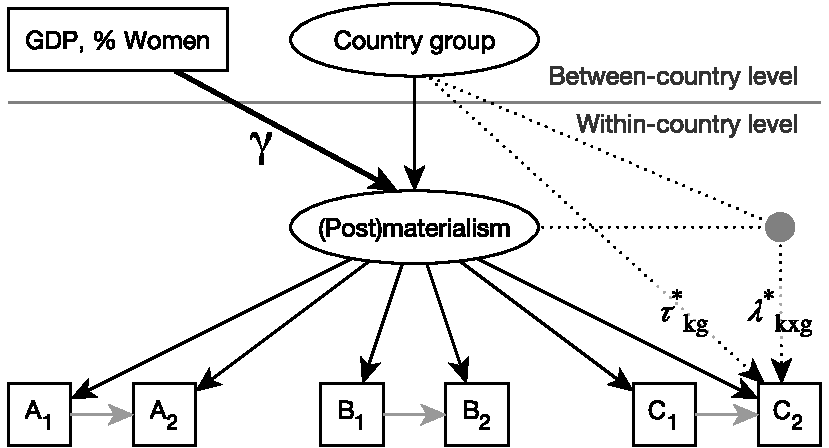
\includegraphics[width=\textwidth]{model}
	\caption{Structural equation model of relationships of interest between four latent variables.
		The regression coefficient estimates shown are averages 
	over all 19 countries under 
	the full metric invariance model (see Figure \ref{fig:davidov-coefficients} for country estimates).
	}\label{fig:davidov-model}
\end{figure}

Data were obtained from the European Social Survey 2002, a 
high quality cross-national probability survey  \citep{jowell_measuring_2007}.
Each latent variable is measured with multiple observed indicators. 
\citet{davidov2008values} compared 19 countries on these regression
coefficients: 
Austria 
($n=$2,257), Belgium  (1,899), Czech Republic 
(1,360), Denmark  (1,506), Finland  (2,000),
France  (1,503), Germany  (2,919), Great
Britain  (2,052), Greece (2,566), Hungary
 (1,685), Ireland  (2,046), Netherlands 
(2,364), Norway  (2,036), Poland  (2,110),
Portugal  (1,510), Slovenia  (1,519), Spain
 (1,729), Sweden (1,999), and Switzerland
 (2,037).
For the original data, precise wording of the
questions, and further information on data collection procedures, we refer to
the ESS website.\footnote{%\url
{http://ess.nsd.uib.no/ess/round1/}}
The left-hand side of Table \ref{tab:descriptives} presents
descriptive statistics for the 17 observed variables. 
The within-country and between-country standard deviations
call attention to  the considerable between-country variation in the means,
which could reflect substantive
differences between the 19 countries, but could also originate in cross-country
loading (or intercept) differences.

\begin{table}\begin{small}
\caption{Left: descriptive statistics for the observed variables. 
	Overall means over countries, 
	within-country standard deviation, and between-country 
	standard deviation.
	Right: loading estimates in the full metric invariance model.}\label{tab:descriptives}
\begin{tabular}{rrp{1cm}p{1.3cm}p{1.3cm} c p{1.15cm}p{1.15cm}p{1.15cm}p{1.15cm}}
  \hline   \hline
 && Overall mean & Within-country sd. & Between-country sd. &&    Self-trans 1. & Conserv. 2. & Allow 3. & No cond. 4.  \\ 
  \hline
1. &  Equality & 2.07 & (1.04) & (0.18)   &	& 0.648 &  &  &  \\ 
2. &  Understanding & 2.41 & (1.05) & (0.18)  &	& 0.711 &  &  &  \\ 
3. &  Environment  & 2.13 & (0.99) & (0.19)  &	& 0.697 &  &  &  \\ 
4. &  Helping others & 2.31 & (0.99) & (0.16)  &	& 0.734 &  &  &  \\ 
5. &  Loyal to friends & 1.97 & (0.89) & (0.19)  &	& 0.647 &  &  &  \\ 
                                       \\
6. &  Modesty & 2.83 & (1.24) & (0.42)  &   &	& 0.677 &  &  \\ 
7. &  Tradition & 2.76 & (1.32) & (0.35)  &   &	& 0.768 &  &  \\ 
8. &  Follow rules & 3.14 & (1.34) & (0.37)  &   &	& 0.847 &  &  \\ 
9. &  Proper behavior & 2.70 & (1.23) & (0.31)  &   &	& 0.920 &  &  \\ 
10. & Security & 2.37 & (1.18) & (0.36)  &   &	& 0.801 &  &  \\ 
11. & Govt. strong & 2.43 & (1.19) & (0.37)  &   &	& 0.838 &  &  \\ 
                                       \\
12. &  Allow other race & 2.54 & (0.78) & (0.27)  &   &  &  & 0.589 &  \\ 
13. &  Allow EU poorer & 2.45 & (0.76) & (0.28)  &   &  &  & 0.612 &  \\ 
14. &  Allow richer & 2.48 & (0.81) & (0.21)  &   &  &  & 0.517 &  \\ 
15. &  Allow poorer & 2.51 & (0.77) & (0.28)  &   &  &  & 0.632 &  \\ 
                                       \\
16.  &  Qualify education & 6.22 & (2.64) & (0.64)  &   &  &  &	&1.732  \\ 
17. & Qualify work skills & 6.75 & (2.65) & (0.78)  &   &  &  &	&2.170 \\ \\
   \hline   \hline
\end{tabular}
\end{small}
\end{table}




Following standard practice, the original authors fit the full metric invariance model
to the ESS data: 
a multiple group structural equation model in which the loadings in Figure
\ref{fig:davidov-model} are constrained to be equal across the 19 countries,
while the structural regression coefficients and other parameters are allowed to vary. 
The right-hand side of Table \ref{tab:descriptives} gives the resulting estimates of 
the loadings (under the variance parameterization). Parameter estimates of interest for the 19 countries  are shown in Figure \ref{fig:davidov-coefficients}. 


\begin{figure}\centering
\includegraphics[width=\textwidth]{Davidov-both-crop.pdf}
\caption{Estimates $\pm 2$ s.e. for the four regression coefficients  between latent variables of interest under the metric invariance model in 19 countries.}\label{fig:davidov-coefficients}
\end{figure}


\citet[589]{davidov2008values} test for (partial) metric equivalence by 
examining overall fit measures as well as 
MI and SEPC-self. They decide that 
``the overall fit measures (CFI = 0.95, NFI = 0.94, RMSEA = 0.01, Pclose = 1.0) suggest that 
[the full metric invariance model] is acceptable. However, modification indices
pointed to misspecifications in the model. Therefore, in model 2 we (...) had to relax the measurement invariance constraints for some items.''
Based on the MI and (S)EPC-self, the author's final model frees four out of 
the possible 323 loading equalities in three different countries, namely ``Conservation $\rightarrow$ Modesty''  in Portugal, 
``Conservation $\rightarrow$ Govt. strong'' in Ireland, and ``Self-transcendence $\rightarrow$ Loyal to friends'' in Portugal and Denmark.\footnote{Davidov (2012, personal communication).} 

The $\da$ statistic provides an alternative way to assess whether a loading equality restriction
is substantively important or not. 
\citet{saris2009testing} suggested a cutoff of 0.1 in absolute value for correlations and standardized regresssion coefficients.
Given the parameterization used, this appears to be a reasonable criterion for the $\da{}$ with respect to regression coefficients as well. 
Although there are potentially 76 affected parameters of interest for each of the 
323 equality restrictions, as it happens only
the four $\da$ statistics shown in Table \ref{tab:davidov-epc} meet this criterion.
The form of the model plays an important role here: equality constraints on 
loadings in one country hardly affect structural parameters in another, 
misspecified constraints on one dependent latent variables' loadings hardly
affect the regression coefficients of the other, and latent variables with
many indicators are generally less affected by misspecifications. 

\begin{table}
\begin{small}
\caption{$\da$ statistics of at least 0.1 in 
	absolute value with respect to the  latent variable regression coefficients. For reference, the standardized expected parameter change (SEPC-self) is also given.}\label{tab:davidov-epc}
\begin{tabular}{llrrrr}
\hline
&& \multicolumn{4}{c}{Loading ``Conditions $\rightarrow$ Qualify work skills'' in...}\\
\cline{3-6}
& & Slovenia  & France  & Hungary  & Ireland  \\ 
\hline
\multicolumn{2}{l}{\emph{$\da{}$ with respect to:}}\\
&Conditions $\rightarrow$ Self-transcendence &	-0.073&	-0.092&	-0.067&	0.073\\
&Conditions $\rightarrow$ Conservation		 &	0.144	&0.139&	0.123&	-0.113\\
\\
\multicolumn{2}{l}{SEPC-self}
	&0.610&          0.692&           0.759       &   -0.514\\
	\hline
	\end{tabular}
	\end{small}
\end{table}


In summary, even though the full metric invariance model shows ``close fit'' in terms of CFI and RMSEA, this model still contains misspecified equality restrictions on loadings that threaten  the comparison of the regression coefficients of interest. Freeing these loadings takes this possibility into account while still allowing for the identification of the parameters of interest. The misspecified restrictions on loadings in question were  not detected with the SEPC-self and MI: these measures detected other misspecifications that were large in the sense of having strongly differing loadings.


\section{Example 3: Sex differences in value priorities}
\label{sec:app3}

Men and women differ in their latent value priorities according to a study by  \citet{schwartz2005sex}, who offered substantive explanations for this finding. Using the European Social Survey 2002 data introduced above, all 21 observed ESS value indicators (see appendix) were modeled as measuring eight factors, following a scheme detailed by \citet{schwartz1987toward}. These ``universal human values'' were: benevolence (BE), universalism (UN), self-direction (SD), stimulation (ST), hedonism (HE), achievement/power (ACPO), security (SE), and conformity/tradition (COTR). 

Before comparing men and women on their latent mean value priorities, the threat of sex differences in response behavior should be ruled out. To this end, a full scalar invariance model was judged to be satisfactory by the authors (p. 1013): 
\begin{quote}\begin{small}
The fit indices for configural and metric invariance were satisfactory (comparative fit index [CFI] = .90, adjusted goodness-of-fit index [AGFI] = .94, root-mean-square residual [RMR] = .07, root-mean- square error of approximation [RMSEA] = .037, confidence interval [CI] = .037�.038, $p$ of close fit [PCLOSE] = 1.0). (...) When we constrained scalar invariance, chi-square deteriorated significantly, $\Delta\chi^2$(19) = 3313, $p$ = .001, but CFI did not change. Change in chi-square is highly sensitive with large sample sizes and complex models. The other indices suggested that scalar invariance might be accepted (CFI = .88, RMSEA = .04, CI = .039�.040, PCLOSE = 1.0).
\end{small}
\end{quote}


I re-analyzed these data, fitting the full scalar invariance model to obtain estimates of the differences between the group of 18,519 men and the group of 16,740 women in their eight latent values factor means. Following the original authors, these sex difference estimates were controlled for age, education level, and country. 

\begin{figure}\centering
	\includegraphics[width=\textwidth]{Schwartz-before-after-crop.pdf}
	\caption{Sex differences in value priorities before and after allowing for 
	between-sex differences in the intercept of ``Important to seek adventures and have an exiting life''.}
	\label{fig:schwartz-before-after}
\end{figure}

Figure \ref{fig:schwartz-before-after} shows estimates based on the full scalar invariance model as red dots. These may be interpreted as latent effect sizes.  Positive values indicate that men value this factor more, while negative values below the dashed line mean women are estimated to value a factor more. It can be seen that Achievement/Power (ACPO), Stimulation (ST), Self-direction (SD), and Hedonism (HE) are estimated to be more important to men, while Security (SE), Universalism (UN), and Benevolence (BE) appear more valued by women. Evolutionary psychology was suggested by \citet{schwartz2005sex} as an explanation for these differences. For instance:  
``stimulation values emphasize and justify the pursuit of excitement, novelty, and challenge in life. Men engage in risky behavior more than women do (...) From an evolutionary perspective, they do this because it serves to increase their social status'' (p. 1021).

It may appear that such conclusions on sex differences in human values are protected from the threat of the alternative explanation that men and women answer the questions differently by the ``closeness'' of the full scalar invariance model fit as evidenced by CFI, RMSEA, etc. But ``close fit'' does not guarantee invulnerable substantive conclusions. Sex difference estimates may change when misspecified intercept equality restrictions are freed--the question is how much. The $\da{}$ for the change in Stimulation's latent mean difference after freeing the  intercept equality restriction on  the item (\emph{Adventure}) ``important to seek adventures and have an exiting life'' is -0.243, for example. Since the effect size estimate in Figure \ref{fig:schwartz-before-after} of this sex difference is +0.214 (s.e. 0.0139) under the full scalar invariance model, the $\da{}$ indicates that freeing this intercept equality has the potential of reversing the conclusion: women would be estimated to value Stimulation more under the alternative model that frees this misspecification, according to the $\da{}$. 

As detected by the $\da{}$, freeing this intercept equality in an alternative model does indeed reverse the conclusion on Stimulation: estimates of the sex differences in latent means after fitting this alternative model are shown as blue triangles in Figure \ref{fig:schwartz-before-after}. The improvement  in model chi-square relative to full scalar invariance (likelihood ratio test) is $\chi_1^2 = $ 827 ($p < 10^{-6}$). It is immediately apparent from Figure \ref{fig:schwartz-before-after} that freeing the intercept of item \emph{Adventure}, which measures Stimulation, changes the estimate of sex differences in that factor. For Stimulation, although the effect size estimate of -0.021 (s.e. 0.014) does not differ significantly from zero, conclusions would now be reversed, women valuing Stimulation more than men: a different evolutionary explanation may have to be found.

In short, the original authors, encouraged by ``close fit'', assumed scalar invariance, concluded that men value Stimulation more than women and theorized that this was due to natural selection of men who take risks. $\da{}$ estimates for the scalar invariance model warn that different assumptions with the same data permit the researcher to conclude the opposite.



%``Greater male competitiveness is also consistent with the higher importance that men attribute to achievement and stimulation values. Achievement values�seeking personal success through demonstrating competence according to social standards�relate directly to competition. Stimulation values emphasize and justify the pursuit of excitement, novelty, and challenge in life. Men engage in risky behavior more than women do (Byrnes, Miller, \& Schafer, 1999). From an evolutionary perspective, they do this because it serves to increase their social status (Wilson \& Daly, 1985).'' (p. 1021)

%``For women to maximize their return on their greater investment in pregnancy, nursing, and caring for infants, concern for the welfare of close others, expressed in benevolence values, would be adaptive. The greater need of women to protect themselves and their infants during the vulnerable period of early child rearing may also make security values that concern safety, harmony, and stability more important to women than to men.'' (p. 1021)

%``Social role theory can explain the greater importance attributed by men than women to achievement, self-direction, and stimulation values by noting the differential placement of the sexes in the occupational world. Men more frequently occupy higher status, money-earning, provider roles that encourage developing skills and values relevant for such work (Valian, 1998). There are also cross-culturally consistent gender role expectations for men to exhibit agentic traits (e.g., Diekman \& Eagly, 2000). Achievement (and power) values justify and give coherence to such agentic behavior as assertiveness, ambition, dominance, and decisiveness. Valuing self-direction does the same for such agentic behavior as self-reliance, independence, and innovativeness. Furthermore, valuing stimulation does this for being active, energetic, and taking initiative'' (p. 1022)

%``In most societies, women's smaller size, lower status, and greater dependence on others' support make them more vulnerable than men. This experience can explain why women ascribe more importance to security values.'' (p. 1022)





%  Try new things~1.g2 Adventure~1.g2 Security~1.g2 Govt. strong~1.g2 Helping others~1.g2
%BE~1.g2          .            .            .             .           0.059
%UN~1.g2          .            .            .             .           .    
%SD~1.g2          .            .            .             .           .    
%ST~1.g2          0.233       -0.205        .             .           .    
%HE~1.g2          .            .            .             .           .    
%ACPO~1.g2        .            .            .             .           .    
%SE~1.g2          .            .            0.087        -0.08        .    
%COTR~1.g2        .            .            .             .           .    

\section{Discussion and conclusion}

%%% Bayes

%In this example, it cannot be ascertained whether or not the intercept in question should be allowed to differ over groups or not. Sensitivity analysis using the $\da{}$, does, however, warn the researcher of the dangers posed by the scalar invariance model's misspecifications. Such a warning or a lack thereof should at the very least be communicated to the reader of the conclusions, and it appears likely that the currently analyzed data set does not suffice to  prove support for the evolutionary explanation.

Invariance of measurement parameters is a requirement for cross-group comparisons of structural SEM parameters with the purpose of ruling out confounding of measurement differences with structural differences. However, as shown in the second column of Table \ref{tab:misspecification}, when the invariance model does not fit the data, this need not necessarily invalidate the comparison of interest. The first two example analyses, which unnecessarily discarded data or freed parameters, attested to this point. Moreover, as also shown in Table \ref{tab:misspecification}, the invariance model may appear to fit well -- leading the researcher to ignore certain ``small'' misspecifications -- even though disregarded misspecifications can still have a substantial impact on the comparison of interest. In the third example, the differences between men and women in their valuation of ``Stimulation'' was estimated as being either positive or negative, depending on whether an intercept was freed over groups or not. That intercept's equality had appeared to fit ``closely'' in earlier analyses, however, possibly due to the large sample size. 

In these examples, and in a small simulation study, the $\da{}$ statistic was found to provide a reasonable measure of whether misspecifications in 
invariance constraints are substantively relevant. 
It approximates the change in parameters of interest if equality-constrained measurement
parameters were freed. 
\texttt{R} code \citep{Rlanguage} implementing the $\da$ for the SEM library \texttt{lavaan} \citep{rosseel2012lavaan} and allowing for reproduction of the examples discussed in this paper is available online at \url{http://hdl.handle.net/1902.1/21816}.

\vspace{12pt}

Although I am confident in the demonstrations given here, the simulation study was not meant to provide a full evaluation under a wide range of realistic conditions. Such an evaluation may provide more insight in the application of the $\da{}$. Similarly, a systematic comparison of its practical application with that of other invariance testing methods for a large range of topics, measurement models,  structural models, misspecifications, and parameters of interest was necessarily outside of the scope of this paper.

A disadvantage of the univariate $\da{}$ measure used is that the measurement parameters in latent variable models are often dependent, meaning that the $\da{}$ suffers from
similar problems of stepwise model improvement and possible 
capitalization on chance as the EPC-self and MI;
\citet{maccallum1992model} discussed these problems, noting that modifications 
in step-wise improvement made without the aid of theory often do not replicate across samples, and that cross-validation could not provide a solution, although
more positive results when using MI and EPC were found by  \citet{kwok2010using}, \citet[ch. 7]{king2011unbiased}, and \citet{whittaker2012using}, while \citet{hancock1999sequential} suggested a method of controlling type-I error that may apply to the test of no change.
Furthermore, \citet{hancock2009tenuousness} showed that the question of ``which'' loading or intercept in a multiple group SEM is invariant is often not identifiable from the data, but that this need not matter for the comparison of substantive interest.
Although these problems are not specific to the $\da{}$, they 
remain a concern. 
One topic for future study is therefore the degree to which the stability problems of stepwise model improvement extend to the $\da{}$. 

When stability of the schoice of invariant measurement parameters is evaluated, it should likewise be evaluated whether the final comparison made differs across samples. That is, the extent to which situations (2) and (3) of Table \ref{tab:misspecification} are indeed prevented. After all, the goal of the $\da{}$ is not to detect precisely \emph{which} measurement parameters are non-invariant, but rather if and how a comparison of structural parameters across groups is warranted. It is not clear whether this goal would be as unstable across samples as the decision on invariance of particular measurement parameters.

%A possible extension to the $\da{}$ would be to evaluate the effect of freeing several restrictions at a time, i.e.--a multivariate version. It is not known, however, to what degree such a statistic continues to perform well both asymptotically and in finite samples. More work  is therefore needed to evaluate the performance of the $\da$, EPC-self, MI statistics, and possibly their multivariate versions for the particular purpose of partial invariance testing.

This article only considered application of the $\da{}$ to scalar and metric invariance, that is, to equality constraints across groups. It was assumed that the basic model held at least approximately, that is, that configural invariance held. Structural parameters are, however, likely to be even more sensitive to configural invariance than to equality restrictions. For example, \citet[Table 1]{yuan2003assessing} showed that large biases in structural variance parameters can occur due to relatively small misspecification in correlated errors. Cross-loadings are likely to strongly affect structural regression coefficients. The $\da{}$ has been defined in such a way as to include the possibility of freeing other restrictions than scalar and metric invariance by the choice of $\mathbf{A}_a$ in Equation \ref{eq:delta}. An evaluation of the use of the $\da{}$ in this case would be a useful topic for future study, effectively extending the evaluation made in this paper from scalar and metric invariance to configural invariance.


%\begin{itemize}
% concept of invariance is also in ``meaning'': construct either operates 
%		differently across groups or is not the same construct across groups
%	\item not a property of scale anymore; different depending on analysis; 
%		requires formulating structural and measurement model at same time
%	\item dependency of parameters
%	\item The paper treats ordinal variables as continuous. This makes some sense given that the example you are working with took a similar approach, however, I'd probably raise this as an issue as a reviewer. Ordinal variable approaches are now standard and becoming the norm. Some mention of this issue and how your approach can work with ordinal variable methods would be useful.
%	\item What were to happen if you were to test a much larger subset of restrictions at once? Can you do that with your procedure? It seems that while any individual restriction might not have a large effect, the effect could be much larger for a subset.
%\item Effect of cross-loadings is probably larger
%\item Quality of approx in other circumstances
%\end{itemize}


In the sensitivity analysis approach, partial measurement invariance is no longer a property of a measurement
model, but becomes a property holding only with respect to a particular analysis of
interest. 
Use of the $\da$  for measurement invariance evaluation requires more substantive knowledge and input from the researcher.
Whether this is a drawback or an advantage is up for debate: arguably, invariance is a requirement in comparative research because of
its substantive implications, so substantive implications should guide decisions on 
whether or not equality restrictions are warranted.
As demonstrated by the example analyses, invariance tests do not guarantee that ``closely fitting'' but misspecified restrictions are inconsequential for 
parameters of interest, nor that ``badly fitting'' equality restrictions are substantively relevant. 
The $\da{}$ thus represents a trade-off between higher analysis complexity  and
a greater degree of confidence that the groups are comparable for the purposes at hand.


\bibliographystyle{pa}
\bibliography{/Users/daob/Dropbox/Bibliography/quality}

\end{document}
